%2345678901234567890123456789012345678901234567890123456789012345678901234567890
%%%%%%%%%%%%%%%%%%%%%%%%%%%%%%%%%%%%%%%%%%%%%%%%%%%%%%%%%%%%%%%%%%%%%%%%%%%%%%%%
% MAURICIO ESGUERRA NEIRA
% Ph. D. Thesis
%%%%%%%%%%%%%%%%%%%%%%%%%%%%%%%%%%%%%%%%%%%%%%%%%%%%%%%%%%%%%%%%%%%%%%%%%%%%%%%%
\chapter{RNA Base Steps}
\label{basesteps} 
\bibliographystyle{nar}
The problem of classification of the space of conformations
%configurations?
of RNA  is not  new, see for  example, Olson  1972 \cite{olson1_1972},
Saenger     1984     \cite{saenger1984},     and    Gautheret     1993
\cite{gautheret1993}.  Although only  a few researchers addressed this
problem  before  the  turn  of  the twenty  first  century,  now  this
situation is changing rapidly. The reason for this fast change came in
the year 2000, when a vast amount of RNA structural information became
available  upon the  elucidation of  the  structure of  the 30S  small
ribosomal  subunit  of   \textit{Thermus  thermophilus},  a  bacterial
ribosome  \cite{wimberly2000,  schluenzen2000},   and  the  50S  large
ribosomal subunit of \textit{Haloarcula marismortui}, an archaeal
%\footnote{I emphasize the  phylogeny of rRNA's here since  there is an
%  ongoing discussion among biologists on whether archaea are closer to
%  prokaryotes, or to eukaryotes.}
ribosome \cite{ban2000}.
\begin{figure}[H]
\centering
\includegraphics[scale=0.36]{Chapter2/rna2000_2009copy.png}
\caption{\textbf{Left:} Total number of RNA bases added to the Protein
  Data  Bank (PDB)  between 2000  and  2010 (exponential  fit line  in
  red). \textbf{Right:}  Total number of RNA  structures solved yearly
  by X-ray crystallography between 2000 and 2010 (exponential fit line
  in blue).}
\label{fig:rnainpdb}
\end{figure}

\noindent Between  1978 and  2000 a total  of 116 RNA  structures with
resolution better than 3.5  \AA, and comprising around 5500 nucleotide
bases were added to the Protein  Data Bank (PDB), and between 2000 and
today  931  RNA\index{RNA}  structures comprising  491,158  nucleotide
bases.  That  is, the increase in  information due to  the solution of
large RNA structures, is about two orders of magnitude, as pointed out
by  Noller \cite{noller2005}.   It is  clear  from the  growth of  RNA
structural  information from  2000  until today  that  both the  total
number of RNA structures deposited in the PDB, and the total number of
nucleotide bases in these  structures, is increasing at an exponential
rate  (as can  be seen  from  the exponential  fits of  these data  in
Figure~\ref{fig:rnainpdb}).  It is important  to note that such growth
comes mainly from ribosomal structures which contain 88 percent of all
RNA bases in the PDB.  So,  even though structural interest in RNA has
been growing since ribosomal  structures became available in 2000, and
several Nobel prizes  have been awarded for work  in this field, along
with   the   exciting   possibilities   of   deciphering   large   RNA
\cite{weinberg2009}  structures  other than  the  ribosome, still  the
growth of  the RNA structural field  is far from that  of proteins, if
weighed by  the growth in  diversity of RNA structural  information in
the past decade.  If we look  at the current distribution of the sizes
of  RNA   structures  counted  in   terms  of  the  number   of  bases
(Figure~\ref{fig:rnaranges}), it is clear that there are large patches
of chain lengths where there are no RNA structures whatsoever.

\begin{figure}{h}
\centering
\includegraphics[scale=0.50, angle=-90]{Chapter2/histogram.png}
\caption{Frequency of  nucleotide bases in RNA molecules  found in the
  PDB classified by  the size of RNA molecules. We  define the size as
  the total  number of nucleotide  bases present per  molecule. Notice
  the  areas  in  transparent  blue  boxes, which  are  devoid of  RNA
  molecules.}
  \label{fig:rnaranges}
\end{figure}

That is,  there are no  solved structures of  RNA with roughly  600 to
1400 bases or 1800 to 2700  bases.  The area of non-coding RNA's holds
great promise for  finding structured RNA's in such  length ranges, as
has recently been suggested  by the Breaker group \cite{weinberg2009}.
A  representative   example  of  the  characteristic   ranges  of  RNA
structures  available  to  date  in  the  PDB can  be  seen  in  Table
\ref{tab:rnarange} for structures larger  than 300 bases. A comparison
between  the  total number  of  structures  of  protein, protein  plus
nucleic acid,  DNA, and RNA, available  at the PDB  from the seventies
until today  -- shown in Figure~\ref{fig:allpolypdb}  -- reveals large
differences between  the number of deposited protein  and nucleic acid
structures.  There  is over  an order of  magnitude more  protein than
nucleic  acid.  The  rate  of   growth  of  DNA  vs.   RNA  structural
information  is  also  changing.  RNA  structures  have  been  growing
steadily since the mid-nineties and seem to parallel the growth of DNA
structures.

%The table and Figure 1.1 come from downloading all structures from
%2000, until today that have RNA in the pdb and that have a resolution
%better that 3.0A, they are 460 structures.
\begin{table}[htbp]
\begin{center}
{\small
\begin{tabular}{c|p{5cm}|c|c|c}
\hline
\bf{PDBID} & \bf{Structure Name} & \bf{Phylogenetic Group} & \bf{Number of bases} & \bf{Year} \\ \hline
1l8v & Mutant of P4-P6 Domain of Group I Intron & Eukaryota & 314 & 2002 \\ \hline
3igi & Group II Intron & Bacteria & 395 & 2009 \\ \hline
1fg0 & Central Loop in Domain V of 23S rRNA & Archaea & 499 & 2000 \\ \hline
2nz4 & GlmS Ribozyme & Eukaryota & 604 & 2006 \\ \hline
1xmq & 30S rRNA & Bacteria & 1522 & 2004 \\ \hline
1ffk & 50S rRNA Subunit & Archaea & 2828 & 2000 \\ \hline
\end{tabular}
}
\caption{Some large  RNA structures  ($>$300 bases) elucidated  in the
  last decade.}
\end{center}
\label{tab:rnarange}
\end{table}

\begin{figure}
\centering
\includegraphics[angle=0, scale=0.3]{Chapter2/allmolecules_per_year.png}
\caption{The total number of structures available in the PDB up to the
  end of year 2009.  The scale of  the axis on the left (in black), is
  ten times  that on the right  (in green). The black  y-axis sets the
  scale for the  number of protein structures available  in the PDB up
  to the end of the year 2009. The green y-axis sets the scale for the
  number of molecular structures containing nucleic acids, RNA only in
  red, DNA only in blue, and  protein plus nucleic acid in green.  One
  can clearly see  that the total number of  protein, RNA, and protein
  plus  nucleic acid  structures is  growing exponentially.  The trend
  also  tends to show  that the  number of  DNA structures  is perhaps
  growing linearly  instead of exponentially.  It  is also interesting
  to see  how the  number of  RNA structures really  lifts off  in the
  middle of the  nineties, whereas for DNA the  growth started earlier
  and seems to be constant now.}
\label{fig:allpolypdb}
\end{figure}

\noindent The  conformational information contained  in RNA structures
can  be   examined  from   three  main  perspectives:   an  atom-based
perspective; a bond-based perspective;  and a third, as yet unexplored
to  our knowledge,  rigid-body-based perspective.   In  the atom-based
perspective, either a direct  comparison of backbone atom positions is
made \cite{reijmers2001},  or a comparison of the  distances between a
reduced set  of atoms taken  from the nucleotide backbone,  sugar, and
base  \cite{sykes2005}.  The  bond-based perspective  is  divided into
three main  categories.  The first considers  the spatial arrangements
of  the  consecutive  covalent  bonds  in the  RNA  backbone  and  the
glycosidic bond between the sugar  and base, that is, the six backbone
torsion  angles and one  glycosidic torsion  angle \cite{reijmers2001,
  murray2003,  hershkovitz2003, schneider2004,  hershkovitz2006}.  The
second   considers  the   pseudo-bonds  between   consecutive   P  and
C4$^{\rm{\prime}}$  atoms  and  the  resulting  pseudo-torsion  angles
$\eta$   and  $\theta$   \cite{olson1_1972,   duarte1998,  duarte2003,
  wadley2007} \footnote{The $\eta$  and $\theta$ pseudo-torsion angles
  are determined  by consecutive backbone torsion  angles as described
  by Olson  \cite{olson1980} in relating the  structural parameters of
  polynucleotide chains to virtual bond vectors.}.  The third category
considers the networks of  horizontal hydrogen bonding patterns coming
from  a definition of  interacting edge  boundaries in  the nucleotide
bases \cite{westhof2000,  leontis2002, leontis2006}.  In  this chapter
we study  the rigid-body  based perspective using  clustering analysis
and  discuss the relationship  of these  findings to  other previously
reported perspectives on RNA conformation.

\section{Consensus Clustering of Single Stranded Base Step Parameters}
To  our  knowledge there  has  been  no  classification of  rigid-body
base-step parameters for the RNA  structures now available in the PDB.
It is important to note here that in crystal structures, the RNA bases
are determined  more accurately than  the backbone torsion  angles, as
has been  shown by Richardson  and collaborators from the  analysis of
van  der Waals  steric  clashes.  This  can  be seen  more clearly  in
Figure~\ref{fig:murray},    reproduced    from    Richardson's    work
\cite{murray2003}, where the red and orange dots in the backbone atoms
region (Figure \ref{fig:murray} b) denote steric clashes and the green
and yellow dots in the base atoms region (Figure \ref{fig:murray} a)
denote very good agreement with expected van der Waals distances.
\begin{figure}[htbp]
 \centering
 \includegraphics[scale=0.4]{Chapter2/murray2003.png}
 \caption{Comparison of base vs.  backbone structure in RNA reproduced
   with  permission  from Jane  Richardson  \cite{murray2003} and  the
   publisher. Here the blue and green dots in (a) denote very accurate
   van der Waals distances, and the  red, pink, and orange dots on (b)
   denote steric  clashes, that  is, distances outside  the acceptable
   van der Waals range.}
 \label{fig:murray}
\end{figure}

\subsection{Combining Fourier Averaging Results and Clustering Analysis}
We   used   standard   clustering   analysis  (CA)   techniques   (see
Appendix~\ref{appendix_a})  to  classify  18  non-ARNA, and  two  ARNA
dinucleotide steps identified  by Schneider at al.\cite{schneider2004}
from  grouping torsion angles  of rRNA  structures in  the 23S
ribosomal  RNA   subunit  (PDB\_ID:1JJ2).   Here   we  describe  these
structures   using  their   base-step  parameters,   that   is,  three
translational parameters  (Shift $D_x$, Slide $D_y$,  Rise $D_z$), and
three   rotational  parameters  (Tilt   $\tau$,  Roll   $\rho$,  Twist
$\omega$), in a hexaparametric vector $\nu$:
\begin{gather}
\nu = (D_x, D_y, D_z, \tau, \rho, \omega)
\end{gather}
The    results,    illustrated   in    the    dendrogram   shown    in
Figure~\ref{fig:eucl_cons},  were  obtained  by performing  clustering
analysis and consensus clustering of the 20 structures kindly provided
to  us by Schneider  et al.   \cite{schneider2004}.  Schneider  et al.
obtained    these    structures,     which    are    illustrated    in
Figures~\ref{fig:nonAclus} and~\ref{fig:steps2}, by applying a Fourier
averaging  technique and  lexicographical clustering  to  the backbone
torsion  angles  found in  the  large  23S  subunit of  ribosomal  RNA
(PDB\_ID:1jj2).   The methodology  we used  to produce  the dendrogram
follows the  approach taken  by others to  recover the  Periodic Table
classification of the  elements from multidimensional property vectors
of the elements \cite{restrepo2004, restrepo2006}.
\begin{figure}[htbp]
 \centering
\includegraphics[angle=90, scale=0.5]{Chapter2/eucli_cons_nonA-RNA.png}
\caption{Dendrogram  showing   the  results  of   Euclidean  consensus
  clustering of base-step parameter  vectors formed from 18 non-A-type
  and  two A-type  rRNA  dinucleotides obtained  by  Schneider et  al.
  \cite{schneider2004}.  The red rectangles around the branches in the
  tree  have  been  chosen   to  highlight  a  four  group  clustering
  solution. The  height of  the dendrogram represents  the simmilarity
  between dinucleotide  steps across various  clustering methodologies
  described in detail in Appendix \ref{appendix_a}.}
% The  height   is  the   optimal  solution  dissimilarities   to  the
% minimization problem of
% a weighted sum of the euclidean dissimilarities between ultrametrics
% for each clustering solution in the ensemble of solutions which use
% different clustering methodologies.
 \label{fig:eucl_cons}
\end{figure}

\begin{figure}[htbp]
 \centering
\includegraphics[angle=90, scale=0.43]{Chapter2/collageb.png}
 \caption{Molecular images of  non-A-RNA dinucleotide (ApU) structures
   organized by  clusters obtained from consensus  clustering of their
   hexadimensional  base-step parameter  vectors.  The  structures are
   centered  on the  reference frame  of  the adenine  base, with  the
   (shaded) minor groove edge of the rigid block on adenine facing the
   viewer.}
 \label{fig:nonAclus}
\end{figure}

\begin{figure}
\centering
\includegraphics[angle=90, scale=0.48]{Chapter2/collage2.png}
\caption{Top view of the non-A-RNA dinucleotides (ApU) centered on the
  reference frame of adenine with its minor  groove edge oriented
  towards  the bottom  of  the  image and  the  major groove  oriented
  towards the top.}
\label{fig:steps2}
\end{figure}

As is clear  from Figures~\ref{fig:nonAclus} and~\ref{fig:steps2}, the
20 structures  identified by Schneider  et al. fall into  seven unique
groups based  on the relative position  of the base  side groups, here
taken to be an  adenine in the 3$'$ position and a  uracil in the 5$'$
position.   Group I  contains  structure {1}  with  bases stacked  and
base-plane normals pointing in  opposite directions, Group II includes
extended,  unstacked  conformations   with  neighboring  bases  widely
displaced  and oriented  roughly perpendicular  to each  other  in all
cases -- structures {15, 16, 10, 14}. Group III also contains extended
conformations but with the uracil  on the minor-groove edge of adenine
and the bases  perpendicular to one another. The  uracil lies near the
"C8-carbon" of  adenine in these cases  -- structures {8,  9, 17}. The
bases in each  of the conformers in Group IV are  more parallel to one
another but are displaced in  four different ways.  The bases in Group
IVa --  structures {2,  4} -- are  unstacked and neither  parallel nor
perpendicular.  Those in  Group IVb -- structures {18,  19, 20} -- are
closely related to A-RNA with parallel and stacked bases. The bases in
Group IVc  -- structures {11, 12,  13} -- are  parallel but unstacked,
with uracil on  the major-groove edge of adenine.   The bases in Group
IVd -- structures {3, 5, 6, 7} -- are also parallel and unstacked, but
with  the  long axis  (y-axis)  of  uracil  perpendicular to  that  of
adenine.  As  is clear from  Figure~\ref{fig:nonAclus}, the conformers
in subgroups IVc and IVd are  closely related, and the dimers in these
two subgroups are  more closely related to those  in subgroup IVb than
to those in subgroup IVa.

In order  to map the groups,  which were obtained  by clustering, back
into the 23S subunit of the ribosome, we computed the root-mean-square
deviation (RMSD)  between the average  of the step parameters  of each
clustered  group   and  the  step   parameters  of  the   23S  subunit
(PDB\_ID:1JJ2).  Before  computing the  RMSD values we  normalized the
step   parameters  using   the   ratio  between   the  difference   of
step-parameters  to their  minimum value,  and their  range.   This is
expressed in Equation~\ref{eq:normalization}.

The  RMSD  results for  each  group are  show  in  histogram plots  in
Figures~\ref{fig:histo1}, and~\ref{fig:histo2}.

The distribution  of conformer groups  is presented in  an alternative
way in Table~\ref{tab:nonA}, where  we count all base-steps which fall
below an  RMSD score  of 10.  It  is important  to note here  that the
computed  RMSD is  not an  all-atom RMSD,  as is  commonly  used after
superimposition of molecular structures,  but the deviation between an
average  base-step parameter  vector  and each  step  (described as  a
vector) in the 23S subunit, where there is no need for superimposition
since the base-step parameter vectors are computed using a middle step
reference frame between the  step bases \cite{lu2003}.  The reason for
choosing 10 as the RMSD cutoff  value is based on visual inspection of
superimposed  reconstructed structures at  different RMSD  values. For
example, for  Group I; if we  reconstruct the ribosomal  steps with an
RMSD of 10  or less using their base-step  parameter values, we obtain
the  set  of  superimposed  structures  shown in  the  left  panel  of
Figure~\ref{fig:superimpose}.   But if  we reconstruct  the base-steps
using  the set of  parameter values  which fall  within a  larger RMSD
cutoff  value  of   15,  as  can  be  seen  in   the  right  panel  of
Figure~\ref{fig:superimpose},  there  will  be  three  new  structures
(whose  second  base  is  show  in  blue ``clouds'')  in  the  set  of
superimposed structures,  which clearly do  not overlap well  with the
structures which fall  under the lower cutoff value  and therefore are
unlikely candidates for being part of such a conformational group.
  
In  Table~\ref{tab:nonA} we see  that the  total number  of structures
which fall into any of the four conformational groups is 31 percent of
the total number of steps in  the 23S subunit of the ribosome, meaning
that  69 percent  of base-steps  are not  recognized. We  believe this
problem might be  due to three factors: 1) the  A-RNA (Structure 20 in
Figures \ref{fig:nonAclus}  and \ref{fig:steps2}) structure identified
by Schneider  et al.   differs from canonical  A-RNA in that  the rise
value is 4.39 \AA, rather than the standard value of 3.30 \AA obtained
for A-RNA  by Arnott and collaborators  \cite{arnott1973}.  This might
have an effect on the number  of structures which can be grouped under
the A-RNA like Group IVb; 2) we are ignoring the richer classification
of    A-RNA   conformations    described   by    Schneider    et   al.
\cite{schneider2004} by only  using conformers 19 and 20  in Group IVb
and  ignoring the remaining  12 A-RNA-like  conformers, and  3) mixing
results  from Fourier  averaging of  sugar-phosphate  backbone torsion
angles, and base-step parameters consensus clustering, might result in
omission of intermediate base-step conformations which could be highly
populated.

Due to this  problem we chose to investigate the  whole space of RNA
conformations  in the  23S  subunit of  the ribosome  (PDBID\_ID:1JJ2)
using  base-step parameters alone  and clustering  analysis validation
techniques as described in the following section.
%% or it could also be  related to the fact that we  are ignoring the
%% remaining A-RNA related set of structures in Berman and
%% collaborators analysis.

\begin{table}[htbp]
\begin{center}
{\footnotesize
\begin{tabular}{c|c|c|c}
\hline
 & \multicolumn{3}{c}{\bf{RMSD Cutoff Value}}\\ \hline
Group   & \bf{10} & \bf{15} & \bf{20}\\ \hline
I & 3 (0.11) & 7 (0.25) & 7 (0.25)\\ \hline
II & 5 (0.18) & 13 (0.47) & 25 (0.91)\\ \hline
III & 1 (0.04) & 5 (0.18) & 23 (0.84)\\ \hline
IVa & 1 (0.04) & 1 (0.04) & 7 (0.25)\\ \hline
IVb & 807 (29.31) & 1696 (61.61) & 1965 (71.38)\\ \hline
IVc & 9 (0.33) & 22 (0.80) & 41 (1.49)\\ \hline
IVd & 35 (1.27) & 99 (3.60) & 191 (6.94)\\ \hline \hline
Total & 861 (31.28) & 1843 (66.95) & 2259 (82.06)\\ \hline
\end{tabular}
}
\caption{Number of base-steps in the 23S subunit of \textit{Haloarcula
    marismortui} with RMSD values less than or equal to 10, 15, and 20
  between  the  average  base-step  vectors  of  the  four  groups  of
  non-A-type  RNA dinucleotide  conformations and  the  2753 base-step
  vectors  in   23S  rRNA.   The   numbers  in  parentheses   are  the
  corresponding  percentages   computed  with  respect   to  the  2753
  base-steps present in the 23S subunit of the ribosome.}
\label{tab:nonA}
\end{center}
\end{table}

\begin{figure}[htbp]
 \centering
\includegraphics[angle=90, scale=0.5]{Chapter2/RMSDschneider1.png}
\caption{Root mean square deviation of the main four groups show in
  Figure~\ref{fig:nonAclus}. The color of the histograms is the same
  as that of the boxes surrounding the structures of
  Figure~\ref{fig:nonAclus}}
 \label{fig:histo1}
\end{figure}

\begin{figure}[htbp]
 \centering
\includegraphics[angle=90, scale=0.5]{Chapter2/RMSDschneider2.png}
\caption{Root  mean  square  deviation  histograms for  the  subgroups
  present in group  IV.  Since subgroup IVb is  composed of A-RNA like
  conformations we  see in the  upper left histogram that  the highest
  proportion of small RMSD values belongs to this group.}
 \label{fig:histo2}
\end{figure}

\begin{figure}[htp]
 \centering
\includegraphics[angle=0, scale=1.5]{Chapter2/G1at10_15b.png}
\caption{Rigid  block   representation  of  dinucleotide   steps.  The
  major-groove side of the  first nucleotide block is oriented towards
  the  viewer and  colored black.  \textbf{Left:} Drawn  in  blue, the
  block     representing     the      Group     I     cluster     from
  Figure~\ref{fig:nonAclus}. Superimposed  on the Group  I cluster are
  three  structures whose  step-parameter RMSD's  with respect  to the
  Group I cluster  are less than or equal  to 10. \textbf{Right}: With
  an RMSD  less than  or equal to  15 we  "identify" a total  of seven
  structures  from the  ribosome. We  clearly see  that three  of them
  (encircled in cyan blobs) are  farther apart from the original Group
  I  main structure  of  Figure~\ref{fig:nonAclus} which  is drawn  in
  blue.}
 \label{fig:superimpose}
\end{figure}

\subsection{Selection of a Clustering Methodology} 
In order to  analyze our dataset of base-step  parameters we have used
clustering  analysis  methods.   Clustering  analysis methods  can  be
broadly  classified into  two main  categories, either  partitional or
hierarchical.   In  either  case   the  main  problem  one  faces  for
classification  purposes is  that of  deciding the  optimal  number of
hierarchies or partitions  that the analyzed data are  split into.  To
obtain  a criterion for  an optimal  number of  clusters, and  also to
decide which method might be better  for our dataset, we have used two
types of  cluster-validation techniques.   They are known  as internal
measures and  stability measures.  Full details of  the definitions of
such  measures   are  provided  in   the  literature  \cite{handl2005,
  brock2008}  and in  Appendix~\ref{sec:validation}.   To perform  the
validation  analysis  we  used  a cluster  validation  package  called
clValid \cite{brock2008},  which is implemented in  the R \cite{rcite}
statistical analysis package.

In  Figures~\ref{fig:internal} and~\ref{fig:stability} we  present the
results for internal and stability validation of clustering techniques
for the  base-step parameters  in the 23S  ribosomal subunit.   In the
clustering analysis literature  it is customary to use  a variable $k$
to define the number of clusters  which we will be using frequently in
the text.

In  Figure~\ref{fig:internal} we  see the  results from  computing the
validation scores (connectivity, silhoutte  width, and Dunn index) for
cluster groups ranging  from $k=2$, up to $k=80$,  and evaluated using
both, hierarchical (hierarchical, diana) and partitional (kmeans, pam,
som, sota) methods. An optimal connectivity measure must be minimized,
and the average  silhouette width (silhouette) and Dunn  index must be
maximized.  Keeping in mind the previously described optimal trends we
see  that  for   the  three  graphs  shown  in   this  figure  the
hierarchical\footnote{The  hierarchical method can  be carried  out in
  various ways,  for example,  using different metrics,  and different
  grouping methodologies.  In this specific case we are referring to a
  hierarchical method  carried out in the  agglomerative, or bottom-up
  manner, meaning that  we start by grouping pairs  of steps which are
  initially  ungrouped,   and  group  them   progresively  with  other
  ungrouped  steps using  the  average method  criteria (explained  in
  Appendix~\ref{appendix_a}),  which  in turn  depends  on a  distance
  definition  which in  this  case  is that  of  the Euclidean  metric
  (defined in  Appendix~\ref{appendix_a}).}  method (black  trend line
marked  as one.)  performs  better in connectivity and  Dunn index
for the whole range of two to eighty clusters, and it is also the best
performer in silhouette from $k=12$ onwards.

Stability  measures (Figure~\ref{fig:stability})  are well  suited for
highly  correlated  data sets  with  linear  correlation between  many
variables, but they  are not very useful for our  data set since, even
though there is correlation between our variables this only occurs for
shift vs. twist, and rise vs. tilt,  as can be seen from the values in
the    upper   right    corner   of    the   pairs    scatterplot   in
Figure~\ref{fig:pairsnoarna},  that   is,  of  the   fifteen  possible
correlated  pairs,   only  two  are  linearly   correlated,  and  such
correlation  is  not very  strong  since  the correlation  coefficient
values are below 0.95, which  means that 90\% of the variation between
variables can be  explained by a linear relationship  between them. We
include the cluster stability measures for completeness in the cluster
validation scheme.

The    stability   measurements   we    have   computed    (shown   in
Figure~\ref{fig:stability})  are  indicative  of a  better  clustering
methodology the smaller their values.  We have computed three measures
for  each of  the hierarchical  and partitional  methods,  namely, the
average proportion  of non-overlap  (APN), the average  distance (AD),
and the  average distance  between means (ADM).   The details  of such
measures  are   given  in  Brock  et  al.    \cite{brock2008}  and  in
Appendix~\ref{appendix_a}.  As  seen in Figure~\ref{fig:stability} the
method which performs the best  according to the stability measures is
sota (second-order tolerance  analysis) for APN and ADM  since one can
clearly see that  in the corresponding curve in  cyan color and marked
with number  five the  values are smaller  consistenly for  almost the
whole range,  up to $k=70$.   In the case  of the AD measure  the best
performers  (those with smaller  values) are  pam (green  curve marked
with number three) and sota  (cyan curve marked with number five) over
the whole range.  Notice that the hierarchical method follows the same
trend as  the other methods, and  that in general, apart  from the APN
measure and  the sota method,  all methods exhibit a  similar behavior
probably due  to the fact that  our data set is  not highly correlated
(that  is,  the dataset  cannot  be reduced  to  a  smaller amount  of
dimensions).

In all cases  we also see that the best overall  number of clusters is
two,  which is  not surprising  since  we haven't  filtered out  A-RNA
structures  from our  data set.  The two  main groups  are  A-RNA type
base-steps, and non-A-RNA steps.

\begin{figure}
 \centering
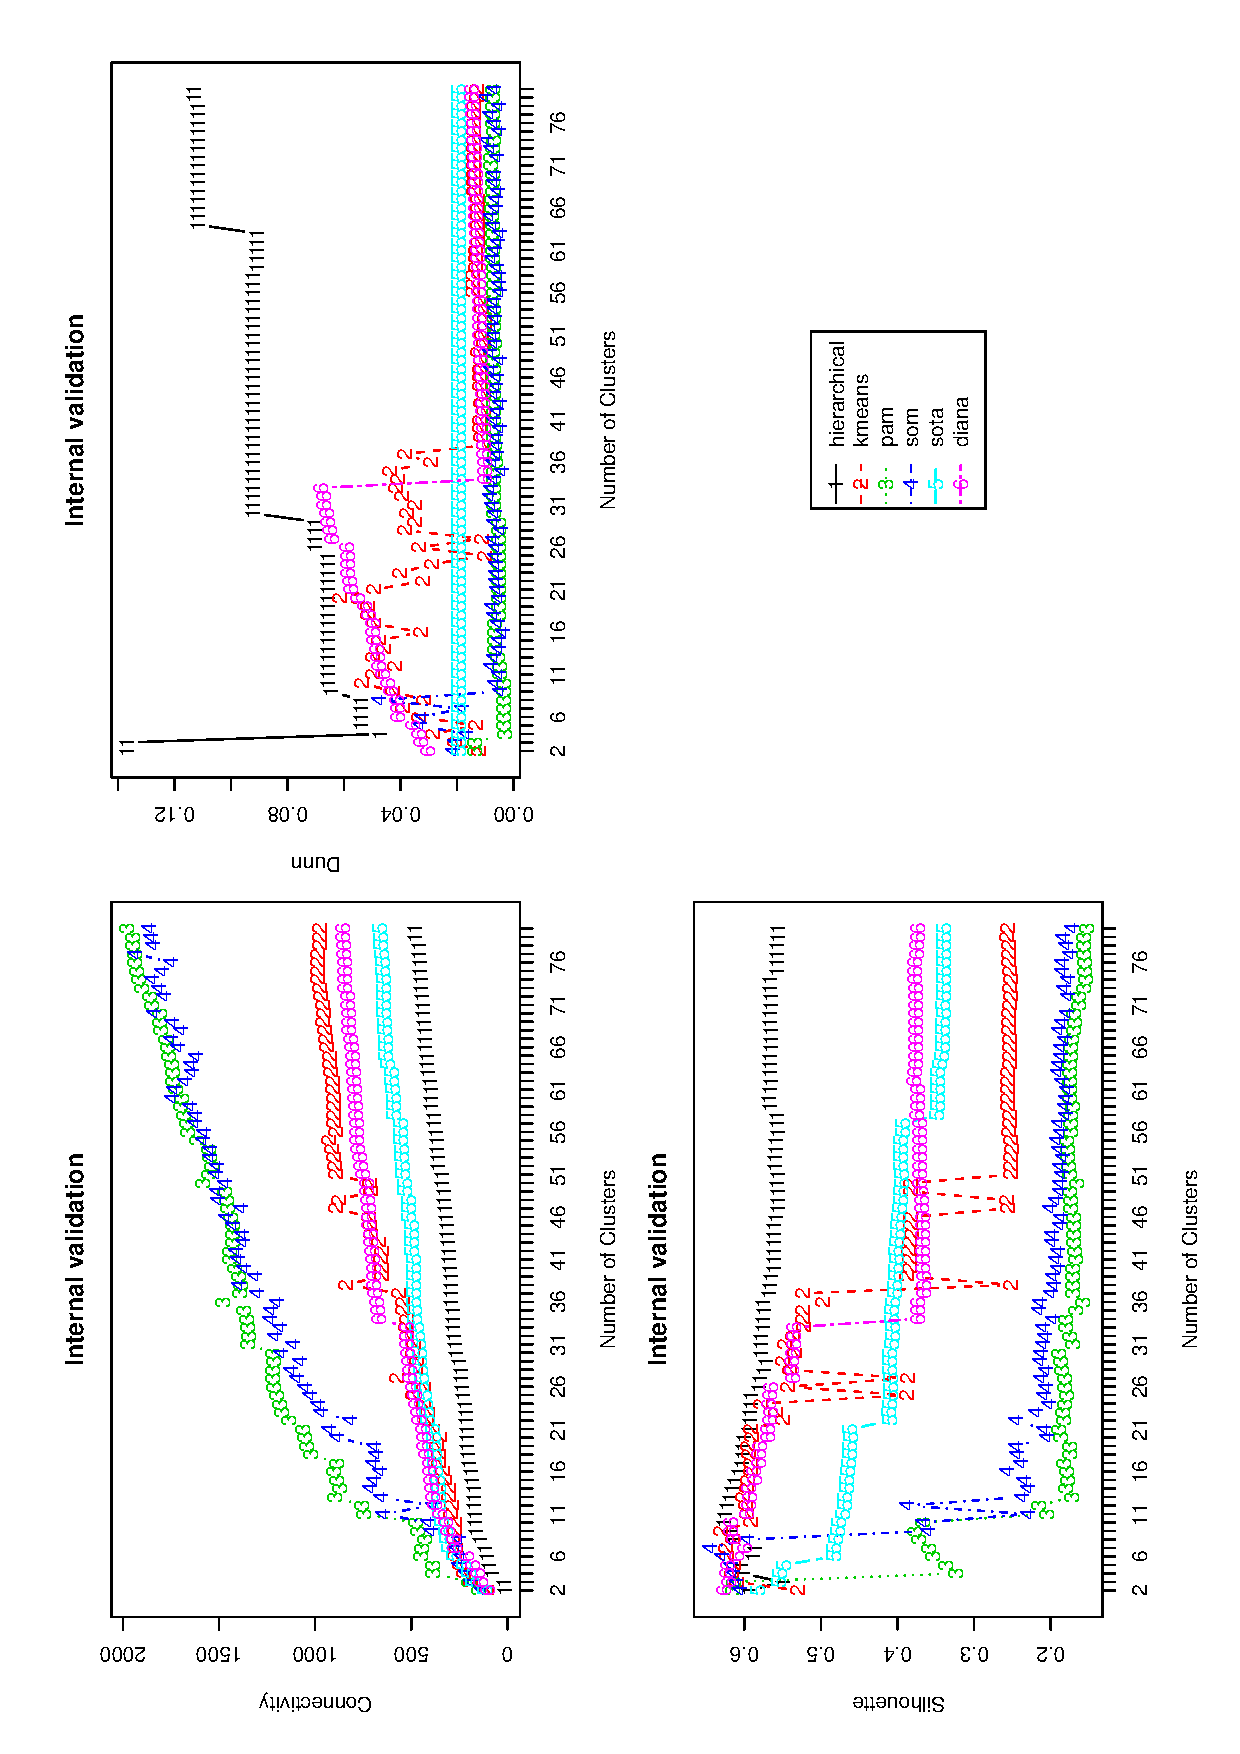
\includegraphics[angle=0, scale=0.34]{Chapter2/STval_int.png}
\caption{Cluster  validity   scores  for  internal   measures  of  all
  base-step   parameters  in   the  23S   subunit  of   ribosomal  RNA
  (PDB\_ID:1JJ2). Notice  how the hierarchical method,  labeled as one
  and drawn  as a black  line, behaves better  for the whole  range of
  connectivity (smaller values) and  Dunn (higher values), and it also
  outperforms all  others after $k=12$ for  silhouette (higher values)
  scores.}
 \label{fig:internal}
\end{figure}

\begin{figure}
 \centering
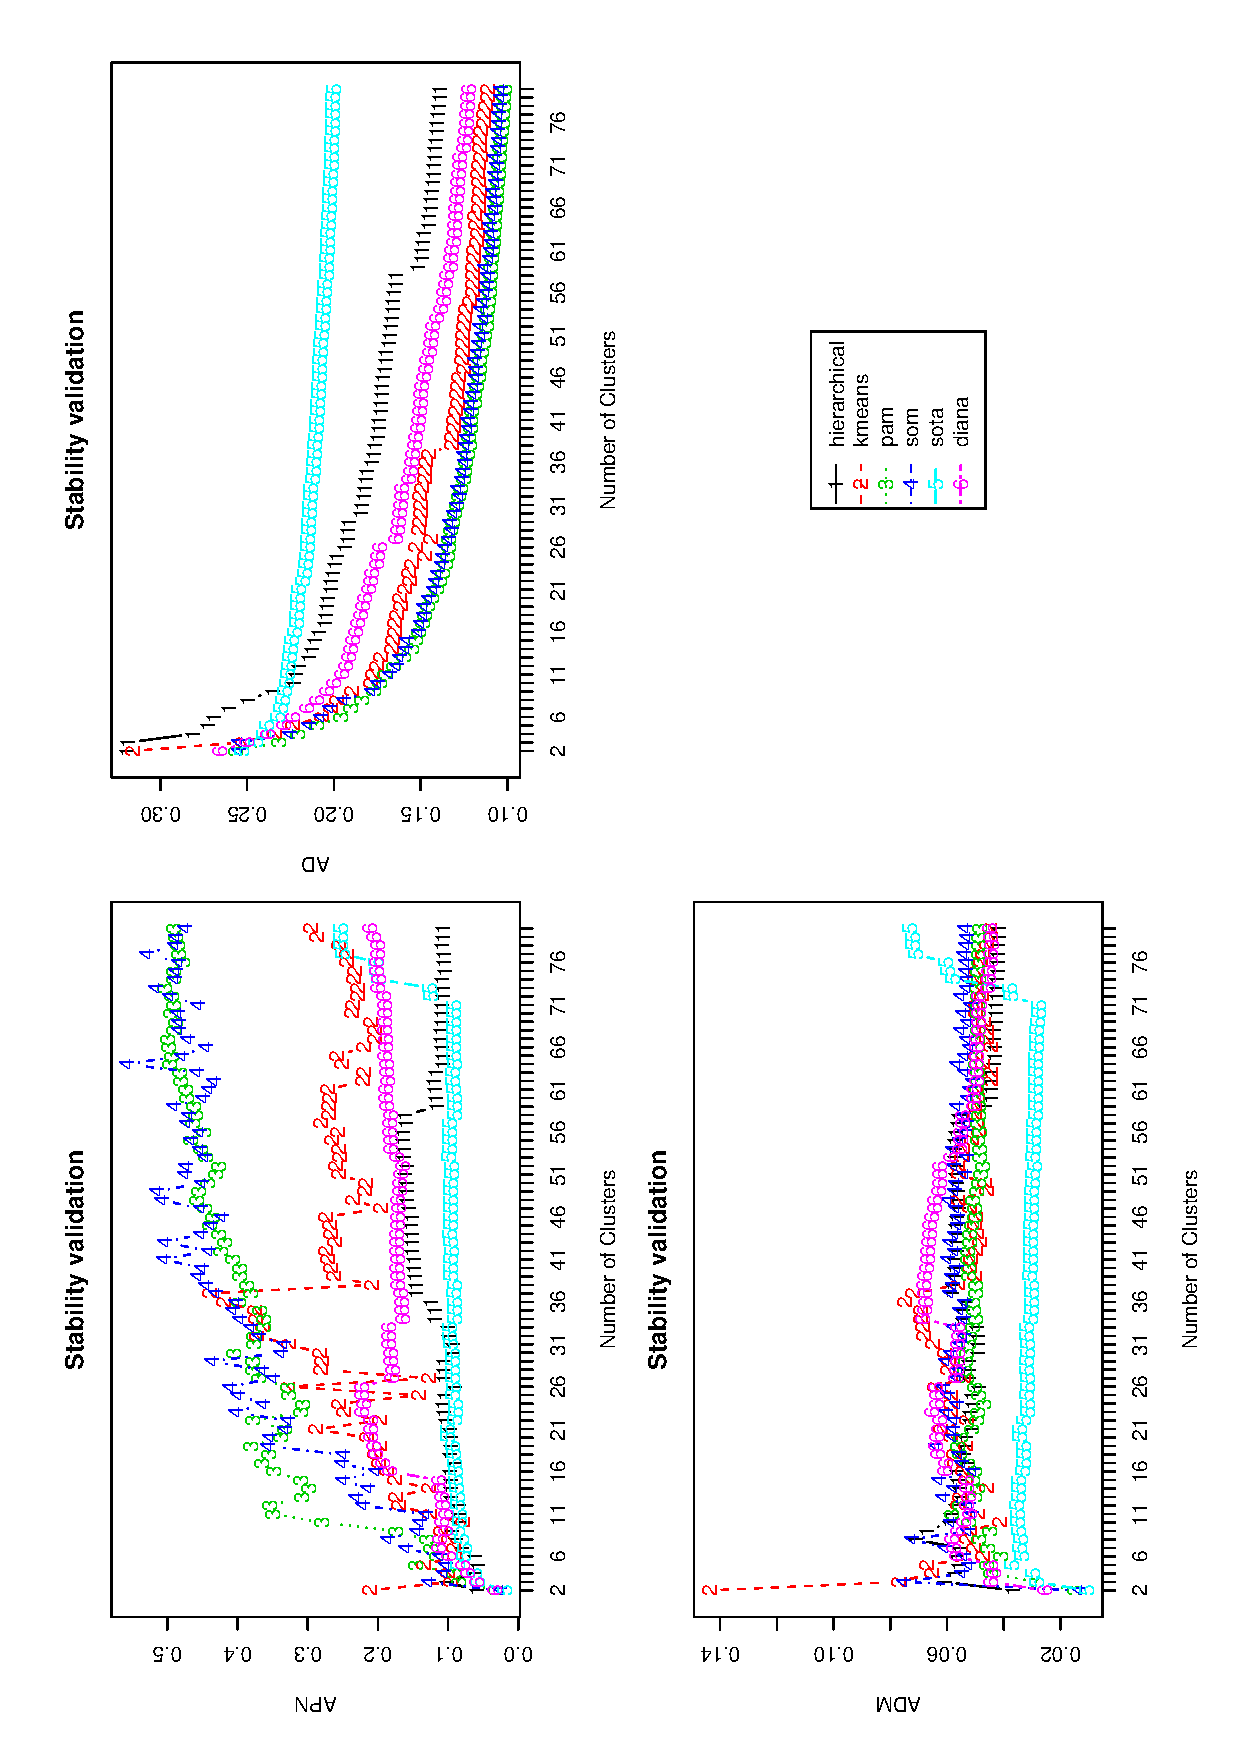
\includegraphics[angle=0, scale=0.34]{Chapter2/STval_sta.png}
\caption{Cluster  validity  scores   for  stability  measures  of  all
  base-step   parameters  in   the  23S   subunit  of   ribosomal  RNA
  (PDB\_ID:1JJ2).  Note that stability measures work specially well for
  datasets of  highly correlated data, which  is not the  case for our
  dataset  but are  shown  here for  consistency  with the  validation
  package clValid.}
 \label{fig:stability}
\end{figure}

We focus  our attention on the  group of structures  which differ from
A-RNA.   We have extracted  797 such  steps (about  29\% of  the total
number  of steps)  from  the  dataset based  on  the root-mean  square
deviation  between step  parameters  (Figure~\ref{fig:dormsd}).  These
base-step parameters are  those with RMSD values greater  than 18 \AA.
These RMSD values have  been computed between the base-step parameters
of  all  dinucleotides  in  the  23S rRNA  subunit  and  the  standard
base-step parameter values of  the canonical A-RNA helix determined by
Arnott   and  collaborators   \cite{arnott1973}  work.   The  standard
base-step parameter values for  common double-stranded RNA and DNA are
listed in Table \ref{tab:conf} .

\begin{figure}[ht]
 \centering
\includegraphics[angle=0, scale=0.38]{Chapter2/dormsd.png}
\caption{Histogram of RMSD values  between base-step parameters of the
  23S subunit  of ribosomal RNA and the  standard base-step parameters
  derived  from  Arnott and  collaborators  \cite{arnott1973} work.  A
  black vertical  line is drawn at  an RMSD value of  18 denoting that
  the  corresponding  base-steps  below  this value  are  assigned  to
  A-RNA-like conformations, and those above this value are assigned to
  non-A-RNA-like conformations.}
 \label{fig:dormsd}
\end{figure}

\begin{table}[ht]
\centering
\small\addtolength{\tabcolsep}{-2pt}
\begin{tabular}{p{1.4cm}|c|c|c|c|c|c|c|c}
\hline
\textbf{Structure Name} & Shift ($D_x$) & Slide ($D_y$) & Rise ($D_z$) & Tilt
($\tau$) & Roll ($\rho$) & Twist ($\Omega$) & \textbf{Reference} &
\textbf{Method} \\ \hline
A-DNA & 0.36 & -1.39 & 3.29 & 2.5 & 12.5 & 30.2 & Arnott
\cite{arnott1999} & fiber-diff. \\ \hline
B-DNA & 0.44 & 0.47 & 3.33 & 4.6 & 1.8 & 35.7   & Arnott
\cite{arnott1999} & fiber-diff. \\ \hline
A-RNA & -0.08 & -1.48 & 3.30 & -0.4 & 8.6 & 31.6 & Arnott
\cite{arnott1999} & fiber-diff. \\ \hline
A'-RNA & 0.05 & -1.88 & 3.39 & -0.1 & 5.4 & 29.5 & Arnott
\cite{arnott1999} & fiber-diff. \\ \hline
AII-RNA & 1.01 & -2.52 & 3.33 & 2.9 & 9.8 & 25.1 & Schneider
\cite{schneider2004} & X-ray \\ \hline
\end{tabular}
\caption{Base    step   parameters    for   common    DNA    and   RNA
  conformations.   The  base-step  parameters   are  computed   for  a
  single-stranded  base-step rather  than a  double-stranded base-pair
  step.}
\label{tab:conf}
\end{table}

\begin{figure}
 \centering
\includegraphics[angle=90, scale=0.48]{Chapter2/warna_step.png}
\caption{Scatterplots for  base-step parameters, shift  (D_{X}), slide
  (D_{y}),  rise  (D_{z}), tilt  ($\tau$),  roll  ($\rho$), and  twist
  ($\omega$), for the A-RNA (colored red) and non-A-RNA (colored blue)
  datasets


  colored   according   to    purine-pyrimidine   (black),
  purine-purine    (red),     pyrimidine-pyrimidine    (green),    and
  pyrimidine-purine (blue) steps. Here the correlation coefficients of
  each of  the scatterplots shown in  the lower half of  the graph are
  listed  in the mirror  position in  the upper  half of  the diagram,
  i.e.,  the  shift-twist  ($D_{x}, \Omega$)  correlation  coefficient
  (0.88)  of the  plotted  data shown  in  the lower  left corner,  is
  printed in the upper right corner.  As seen from the coloring scheme
  there is  no clear  sequence preference for  purine-pyrimidine (RY),
  purine-purine  (RR), or  pyrimidine-pyrimidine  (YY) single-stranded
  steps.}
 \label{fig:allsteps}
\end{figure}

\begin{figure}
 \centering
\includegraphics[angle=90, scale=0.48]{Chapter2/noarna_step.png}
\caption{Scatterplots  for base-step  parameters, shift,  slide, rise,
  tilt, roll, and twist, for the non-A-RNA dataset (taken as the steps
  with RMSD's greater than 18) colored according
  to      purine-pyrimidine     (black),      purine-purine     (red),
  pyrimidine-pyrimidine   (green),    and   pyrimidine-purine   (blue)
  steps. Here the correlation coefficients of each of the scatterplots
  shown  in the  lower half  of  the graph  are listed  in the  mirror
  position in  the upper  half of the  diagram, i.e.,  the shift-twist
  ($D_{x}, \Omega$) correlation coefficient (0.88) of the plotted data
  shown  in the  lower  left corner,  is  printed in  the upper  right
  corner.  As  seen  from the  coloring  scheme there  is no  clear
  sequence preference for  purine-pyrimidine (RY), purine-purine (RR),
  or pyrimidine-pyrimidine (YY) single-stranded steps.}
 \label{fig:pairsnoarna}
\end{figure}

With the filtered dataset, which we refer to as the non-A-RNA dataset,
we  have  again  performed  a  clustering  validation  analysis  using
internal  measures   and  the   computed  results  are   displayed  in
Figure~\ref{fig:nonarna}.  As was the  case for  the whole  dataset of
``A-RNA  like'' and ``non-ARNA-like''  base-steps the  best clustering
methodology to be  applied to the dataset according  to the validation
results, is  the hierarchical  clustering methodology. This  is clear
from   each   one   of   the   validation   score   plots   shown   in
Figure~\ref{fig:noarna},  where the  trend line  for  the hierarchical
method  is show in  black and  marked as  one and  is small  for the
connectivy and  silhoutte scores and  large for the Dunn  index score,
which,  as  stated for  the  case of  the  full  dataset analysis,  is
indicative of an optimal method.

Looking  at the  upper right  plot of  Figure  \ref{fig:noarna}, which
plots the results for cluster  validation using the Dunn index, we see
that the  optimal number of clusters  is $k=67$. The  Dunn index works
under the idea of finding the best possible separation and compactness
(see  Appendix  \ref{appendix_a}  for  definition  of  separation  and
compactness) between clusters, so,  accordingly the result of grouping
the 797  base-steps into 67  groups should produce well  separated and
compact groups. The  other two indices show, as  for the whole dataset
case,  that the  optimal number  of  clusters is  two. Nonetheless,  a
common indicative of optimal cluster solutions in the connectivity and
silhouette  plots is  given by  the presence  of shoulders.  In Figure
\ref{fig:noarna} we  see that there is  a shoulder also  at $k=67$ for
the  connectivity (in  the upper  left) and  silhouette plots  (in the
lower left).

We selected the 67 clusters given by the hierarchical method, and took
their   corresponding  step-parameter   values   to  reconstruct   the
dinucleotide      step       structures      using      3DNA.       In
Figure~\ref{fig:noarnak67} we draw the first seventeen groups with ten
or  more structures,  which account  for 80  percent of  the non-A-RNA
steps.    We    also   plot   in    the   lower   right    corner   of
Figure~\ref{fig:noarnak67} the  set of 20 structures  derived from the
work  of Schneider et  al.\cite{schneider2004}, and  the whole  set of
non-A-RNA  dinucleotide  steps in  a  common  reference  frame on  the
adenine  of  an ApU  step.   All  structures  are centered  using  the
standard  reference frame  embedded in  the first  base, which  in our
reconstructions corresponds  to a red block  representing adenine. The
minor-groove  edge  of  the  adenine  is oriented  to  the  left,  its
major-groove  edge  to  the  right,  and  the  so-called  Watson-Crick
base-pairing edge is pointed toward the viewer.

When comparing the 17 groups of non-ARNA dinucleotide steps with those
found  by Schneider and  collaborators, we  see that  in their  set of
structures there are no steps  represented at the major-groove side of
the red block representing adenine, that is, the right side of the red
adenine  block, although  there are  many  such steps  in the  crystal
structure, we also see, that even though the 17 represented groups
are  not  as compact  as  one  would desire,  they  start  to give  an
indication of the geometrical preferences of the space of dinucleotide
step-parameters.  For  example, it  is remarkable to  see in  Group 7,
labeled as  g7.png in Figure~\ref{fig:noarnak67} that  the cyan blocks
representing  uracil, orient  their planes  orthogonally to  the major
groove side of the red block representing adenine.

The reason we choose to include am image of all non-ARNA base-steps
in Figure~\ref{fig:noarnak67} is that of  giving the reader an idea of
the complexity of the conformation space described from
a  base  viewed  perspective  instead  of  the  more  common  backbone
perspective. This image suggests that the task of finding order in this
broad range of possible conformations is somewhat analogous to solving
a ball puzzle. There are various ball puzzles, but the one which most
resembles this  case is that  of a so-called masterball  puzzle, which
consists of  a sphere with two  parallel lines at  roughly 60$\deg$ of
latitude  north  and  south  from  the  sphere's  equator,  and  eigth
meridians,    as    seen    in     the    left    side    of    Figure
\ref{fig:masterball}. We believe the puzzle can be effectively solved
by using appropriate validated clustering analysis techniques.


\begin{figure}
 \centering
\includegraphics[angle=0, scale=0.72]{Chapter2/noarna_val.png}
\caption{Cluster validity  scores for the non-ARNA dataset.  It can be
  seen  clearly  that  the   optimal  method  for  clustering  is  the
  hierarchical one,  as measured by  lower values in  the connectivity
  scores, and higher  values in the Dunn score.  The optimal number of
  clusters given  by the Dunn  score is 67,  we also see  shoulders at
  $k=67$, for the connectivity and silhouette scores.}
 \label{fig:noarna}
\end{figure}

\begin{figure}
\centering
\includegraphics[angle=0, scale=0.32]{Chapter2/k67_17.png}
\caption{17  out of  the 67  groups clustered  using  the hierarchical
  clustering algorithm are  drawn. Each group is centered  on the base
  reference frame  of the  adenine block drawn  in red.  In  the lower
  right  corner  of  the  "contact   sheet"  the  full  space  of  797
  reconstructed steps is  shown, along with the 20  steps derived from
  Schneider  et al. work.  Notice how  the only  "hollow" side  of the
  "onion" formed by the full  space of base-step conformations is that
  corresponding to the Watson-Crick base-pairing edge.}
\label{fig:noarnak67}
\end{figure}

\begin{figure}
\centering
\includegraphics[angle=0, scale=0.4]{Chapter2/masterball2.png}
\caption{Rebuilt  base-step  parameters  of  the 23S  subunit  of  the
  ribosome using the reference frame of adenine (drawn as a red block)
  in the left side of the figure, resemble a jumbled masterball puzzle
  on the right side.}
\label{fig:masterball}
\end{figure}




\bibliography{biblio}

